\section{Background and Motivation}
\subsection{Post Training Quantization in LLM}
Post-Training Quantization (PTQ) \citep{OBD, OBS, obs2order, gptq, woodfisher} aims to decrease model weight size by simplifying the numerical representation and seeking to maintain the model's accuracy without retraining the model.
We can formulate PTQ as the following optimization problem:
\begin{equation*}
\begin{aligned}
    & \arg\min \quad \mathbb{E} [ \mathcal{L}(\mathbf{X}, \mathbf{W} + \Delta \mathbf{W}) - \mathcal{L}(\mathbf{X}, \mathbf{W})] \\
    & \approx \Delta \mathbf{W}^T \cdot g{(\mathbf{W})} + \frac{1}{2}\Delta \mathbf{W}^T \cdot H{(\mathbf{W})} \cdot \Delta \mathbf{W}
\end{aligned}
\label{eq:exp_optimization}
\end{equation*}
where $\mathbf{W}$ is the original model weights, $\mathbf{\hat{W}}$ is quantized weights, and $\Delta \mathbf{W} = \mathbf{\hat{W}} - \mathbf{W}$ represents the weight quantization error. 
The loss of the model task is $\mathcal{L}$.
The optimization object is to minimize the impact of model quantization on the model task, which means minimizing the expected deviation of the loss function.

PTQ typically employs a concise and accurate method for analyzing the above optimization problem: Second-Order Optimization. Following a Taylor series expansion, this method breaks down the optimization goal into first-order, second-order, and higher-order terms.
$g(\mathbf{W})$ and $H(\mathbf{W})$ represent the gradient and Hessian of task loss $\mathcal{L}$, respectively.
It often assumes that the model has already reached local optimum before model quantization, which means that the first-order term is nearly zero. 
Higher-order terms exert a minor effect on the optimization goal, and we typically disregard interactions among weights between different layers. 
Consequently, we can simplify the optimization problem by focusing on optimizing the second-order term and then define the following optimization problem:
\begin{equation}
\begin{aligned}
    \arg \min_{\Delta \mathbf{W} } \quad & \Delta \mathbf{W}^T \cdot H(\mathbf{W}) \cdot \Delta \mathbf{W}, \\ 
    & \text{s.t. \quad} \Delta \mathbf{W} = \mathbf{0}
\end{aligned} \label{eq:optimization_problem}
\end{equation}
The objective of the optimization problem is to minimize the second-order error in model quantization, subject to the constraint that the change in model weights is as minimized as possible, i.e., $\Delta \mathbf{W} = \mathbf{0}$.







\subsection{Vector Quantization in Neural Networks}
\begin{figure}[t!]
    \centering
    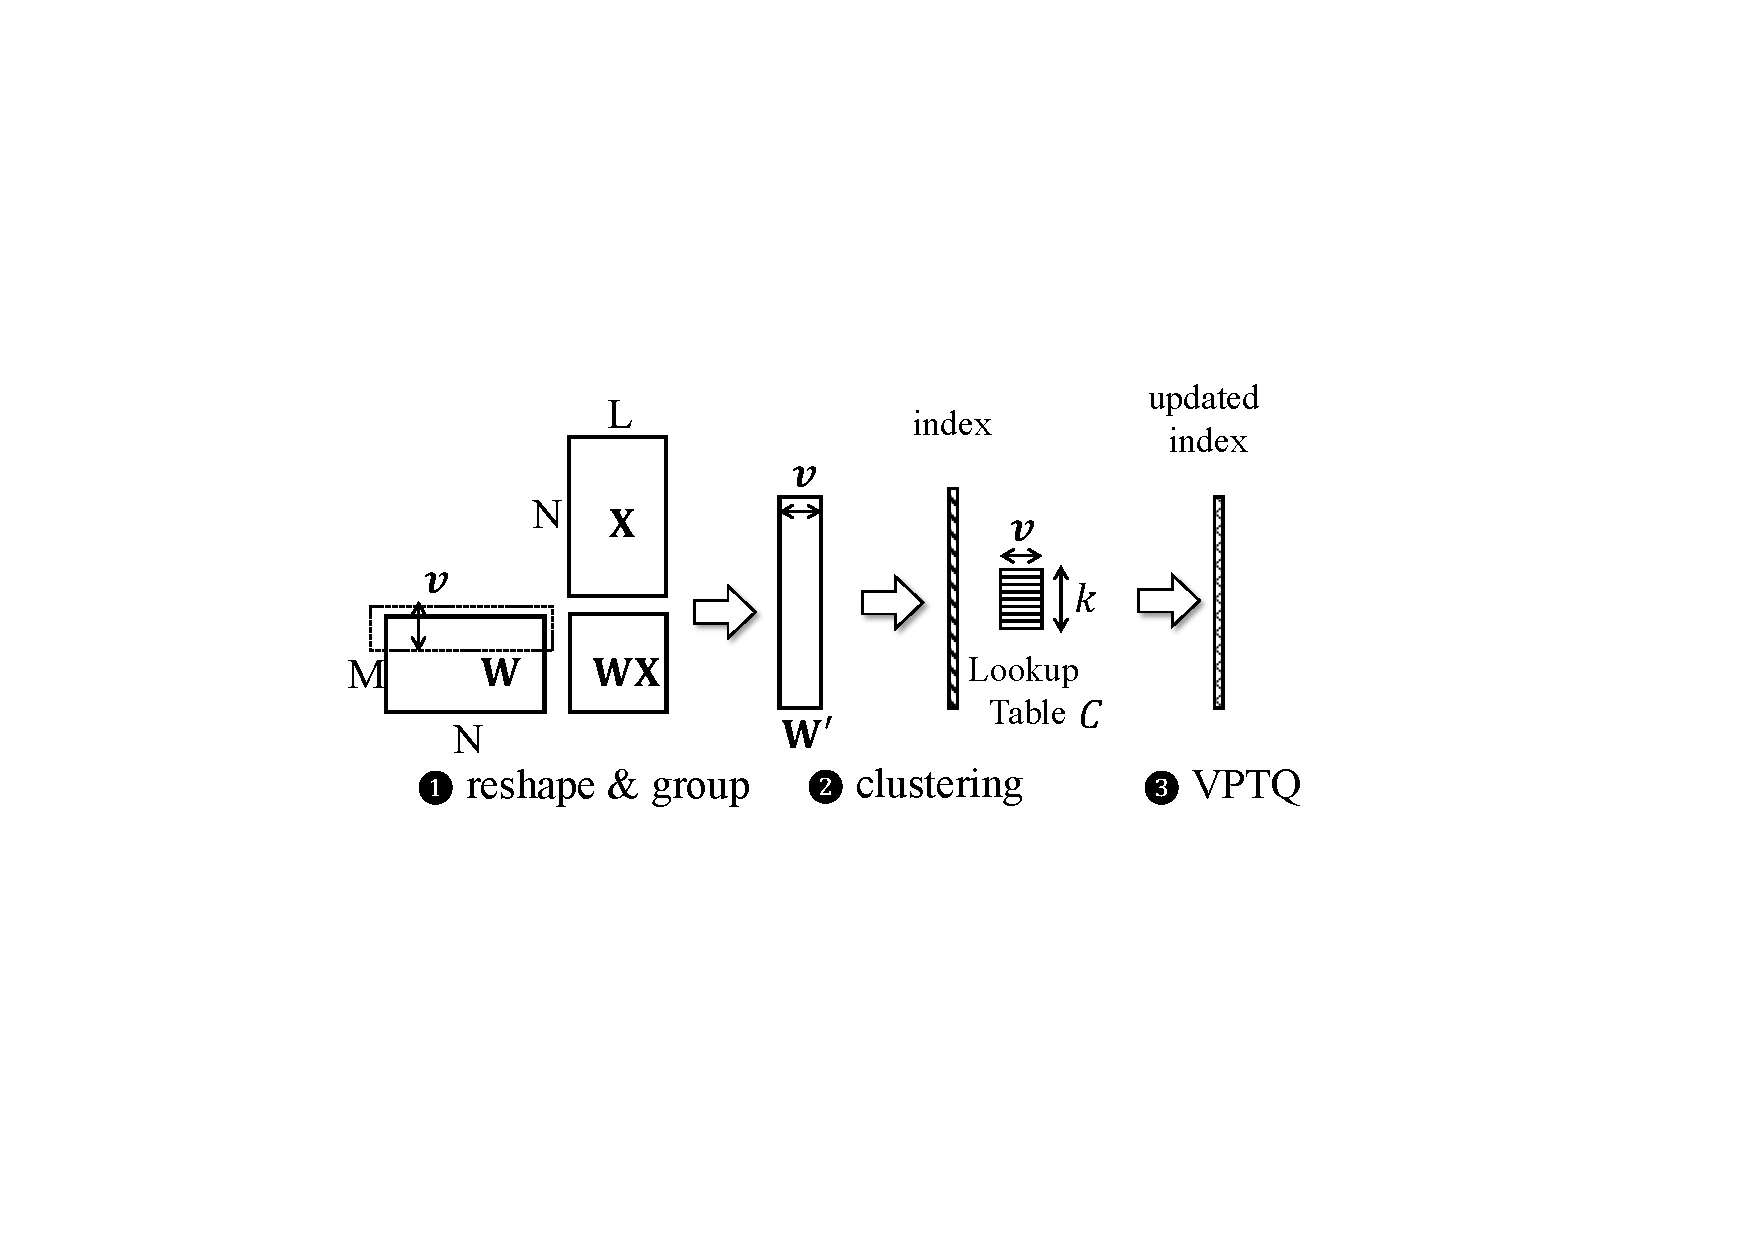
\includegraphics[width=\columnwidth]{figure_tex/vq_example_fixed.pdf}
    \caption{Vector Quantization in Weight Quantization}
    \label{fig:vq_example}
\end{figure}

VQ is a key method for efficient lossy data compression \citep{Gersho}. 
Its objective is to reduce the distortion by mapping high-dimensional original data to a lower-dimensional space represented by a lookup table (Eq. \ref{eq:vq_eq}). 
VQ maps original vectors ($\mathbf{W'}$) from the vector space to a finite set of vectors, which is commonly referred to as a codebook (lookup table, $\mathcal{C}$).
Each vector in the original space approximates the closest vector (centroid $\mathcal{C}_i$) in the codebook.
\begin{equation}
\arg \min_{i \in k} \| \boldsymbol{v} - \mathcal{C}_{i} \|^2, \forall \boldsymbol{v} \in \mathbf{W'}
\label{eq:vq_eq}
\end{equation}
VQ indicates the nearest centroid $\mathcal{C}_{i}$ that minimizes the Euclidean distance between the input vector $\boldsymbol{v}$ in the lookup table. 
The optimization problem aims to find the index $i$ that results in the smallest distance between $\boldsymbol{v}$. 
Thus, each input vector is represented by the most similar centroids, thus minimizing total distortion.





Recent research has explored the use of VQ for model weight quantization \citep{diff-embed-pq, DKM, ABGD, PQ-metaseq}. These studies attempt to compress the embedding layer, the convolution layer, and the classification layer of neural networks using VQ. Figure~\ref{fig:vq_example} illustrates an example of applying VQ to compress model weights on a weight matrix.
For a weight matrix $\mathbf{W}$ with dimensions $M \times N$, we reshape $\mathbf{W}$ into vectors of length $\boldsymbol{v}$ as $\mathbf{W'}$ (step \ding{202}). 
The number of reshaped vectors should be $\frac{M \times N}{\boldsymbol{v}}$.
Next, we employ k-means or other clustering algorithms to build a codebook (step \ding{203}). 
The constructed codebook contains $k$ centroid vectors, each with $\boldsymbol{v}$ dimensions.
Applying the VQ algorithm directly often does not yield an acceptable accuracy. 
Typically, PTQ algorithms adjust the model index and centroid to enhance the accuracy of the quantized model (step \ding{204}).


During model inference, each operator in the model first dequantizes the original weight matrix from the lookup table (codebook) by index and centroid. 
Unlike scalar quantization, VQ keeps the index and centroid in quantized weight. 
The equivalent compression ratio of VQ can be formulated as: $\text{total original model bits} / (\text{codebook bits} + \text{index bits})$. 
The equivalent quantization bitwidth is as: $\text{original bit width}/\text{compression ratio}$.
For example, a $4096 \times 4096$ FP16 weight matrix with vectors of length $v=8$ and $256$ centroids, the compression ratio is $(16 \times 4096 \times 4096) / (8 \times 256 \times 16 + log_{2}(256) \times 4096 \times 4096 / 8) = 15.97$. 
The equivalent bitwidth is $1.002$ bit. 



\subsection{Vector Quantization in LLMs}
While VQ has been applied to weight quantization, the following significant challenges persist when quantizing LLM. 
We summarize the benefits and weaknesses of recent research \citep{AQLM, QuIPsharp, GPTVQ} techniques in Table \ref{tab:intro_table}.

The number of parameters in LLMs is enormous, which requires quantizing the model using lightweight methods to avoid excessive resource consumption.
AQLM \citep{AQLM} utilizes gradient descent to train each layer of the VQ-quantized model and simultaneously trains across multiple layers using calibration data.
It achieves effective compression through additive quantization and joint optimization of the codebook, which can achieve high accuracy. However, due to AQLM's use of backpropagation for model training, significant GPU hours and memory are required to achieve better accuracy, especially when dealing with LLMs with massive parameters.

GPTVQ \citep{GPTVQ} utilizes the Second-Order Optimization method to implement PTQ. 
However, GPTVQ accumulates quantization errors within vector quantization, leading to an inevitable increase in quantization errors as the vector length increases. 
It prevents the use of longer vectors and consequently limits the compression ratio.

QuIP\# \citep{QuIPsharp} introduces an incoherence processing using the randomized Hadamard transform for the weight matrix before VQ. 
The processed weight matrix approximates a sub-Gaussian distribution, allowing for compression with a tiny codebook.
However, incoherence processing requires a significant amount of computation, despite QuIP\# being able to compress LLM to extremely low-bit with a low accuracy drop.
It requires significantly more computation for inference compared to the original LLM, resulting in low inference throughput.











